\documentclass[11pt]{article}
\usepackage[margin=1in]{geometry}
\usepackage{amsmath,amssymb,amsthm,mathtools}
\usepackage{graphicx,booktabs}
\usepackage[colorlinks=true,linkcolor=blue,citecolor=blue,urlcolor=blue]{hyperref}
\newtheorem{theorem}{Theorem}
\newtheorem{proposition}[theorem]{Proposition}
\newtheorem{lemma}[theorem]{Lemma}
\newtheorem{corollary}[theorem]{Corollary}
\theoremstyle{definition}
\newtheorem{definition}[theorem]{Definition}
\newtheorem{hypothesis}[theorem]{Hypothesis}
\theoremstyle{remark}
\newtheorem{remark}[theorem]{Remark}
\newcommand{\ket}[1]{|#1\rangle}
\newcommand{\bra}[1]{\langle #1|}
\newcommand{\braket}[2]{\langle #1|#2\rangle}
\newcommand{\Hel}{\mathrm{Hel}}
\newcommand{\Prod}{\mathrm{Prod}}
\newcommand{\MPS}{\mathrm{MPS}}
\newcommand{\E}{\mathbb{E}}

\title{When does the Past Hypothesis select the subsystems?\\ Quantum mereology as constrained tomography}
\author{[Author name(s) and affiliation(s) --- to be completed]}
\date{Draft, September 2026}

\begin{document}\emergencystretch=2em
\maketitle

\begin{abstract}
In Hilbert-space fundamentalism the world is a Hamiltonian $H$ and a state $\psi$, and the division into subsystems must be derived. Stoica has shown that no such derivation can be unique: every tensor product structure (TPS) in which $H$ is local is one of a continuum related by unitaries commuting with $H$. We show that imposing a strengthened form of the Past Hypothesis as a selection rule --- choose the division in which some moment of the history is simple (close to a product state, or to a matrix product state) --- reduces the preferred-structure problem to constrained quantum state tomography: recovering the simple moment of the history (the \emph{bounce}) from a single projective measurement in the energy eigenbasis, with simplicity as prior information. Known results on constrained tomography then imply that, for a generic eigenbasis and an exactly simple bounce, the rule selects the actual history uniquely up to time translation, a residual freedom whose significance is itself debated. For Haar-random eigenbases we prove a robust version with explicit constants, covering bounces close to matrix product states and hence area-law states with extensive entanglement, for any spectrum, including the commensurable spectra recently proposed to avoid Boltzmann brains. For local Hamiltonians we show that central-limit-level information about energy distributions cannot separate simple states that differ locally, and that under an eigenstate-thermalization-type hypothesis simple states are separated in expectation. The uniform separation the rule needs is open; simulations of chaotic spin chains of up to 12 qubits support it at high energy. The selection is thus proved for generic and random eigenbases and conjectural for local Hamiltonians. For time-reversal-invariant Hamiltonians we prove the analogous exact statement with time reversal added to the residual freedom: the rule fixes the history but not its direction.
\end{abstract}

\section{Introduction}
\label{sec:intro}

Hilbert-space fundamentalism (HSF) holds that the only fundamental data are a Hilbert space, a Hamiltonian $H$ and a state $\psi$, and that everything else --- in particular the factorization of the Hilbert space into subsystems --- emerges from them~\cite{CarrollSingh2021,Stoica2022}. That subsystems are relative to a choice of observables goes back at least to Zanardi, Lidar and Lloyd~\cite{ZLL2004}. The factorization problem has been approached through locality of the Hamiltonian~\cite{CPR2019}, quasi-classical dynamics~\cite{CarrollSingh2021}, operational criteria such as minimal scrambling~\cite{Zanardi2024}, searches for classical subsystems~\cite{Adil2024}, unitary invariants of the pair $(H,\psi)$~\cite{Soulas2025}, and spectral data more generally~\cite{LoizeauSels2024,Cao2026,Kushwaha2026}. Stoica has argued that these programmes cannot succeed as stated: any structure built from $(H,\psi)$ alone in a unitarily covariant way is non-unique, because the torus $\Gamma$ of unitaries commuting with $H$ maps one local TPS to a continuum of equally local ones, and the state reads differently in each~\cite{Stoica2022,Stoica2024,Stoica2026}. Soulas, Franzmann and Di Biagio have replied that a TPS can be fixed by suitable invariant properties of $(H,\psi)$, while conceding that their construction lacks direct physical meaning~\cite{Soulas2025}; Stoica maintains that such properties amount to fixing the structure by hand~\cite{Stoica2026comment}.

Two further observations frame this note. First, for generic spectra the time-evolution orbit is dense in $\Gamma$, so every alternative local TPS is a limit of time translates; alternative divisions then amount to other times rather than other worlds (Stoica~\cite[Remark~11]{Stoica2022}, credited to D.~Ranard). Second, Carroll, Diachenko and Dulani have proposed a finite-dimensional cyclic cosmology whose commensurable spectrum makes the history a closed loop, precisely to avoid Boltzmann brains~\cite{CDD2026}. In that setting the loop has measure zero in $\Gamma$, so almost every alternative local TPS reads the state as one the history never visits. The escape from Boltzmann brains therefore reopens the ``which world'' form of the non-uniqueness problem.

\paragraph{Contributions.} We study a selection rule based on a strengthened form of the Past Hypothesis: the requirement that the history contains a \emph{simple} moment, which we call the \emph{bounce}. This is a substantive postulate about the early state, close to the Entanglement Past Hypothesis~\cite{AlKhaliliChen2024} and stronger than low thermodynamic entropy. Stoica already considered the Past Hypothesis for this purpose and argued that it cannot give uniqueness~\cite[Sec.~VII.B]{Stoica2022}. We show that, among locality-preserving divisions, it gives uniqueness up to time translation (and, for time-reversal-invariant Hamiltonians, time reversal), the case Stoica identifies as yielding a unique spacetime~\cite[Remark~10 and Sec.~VII.E]{Stoica2022}.
\begin{enumerate}
\item \emph{Reduction (Sec.~\ref{sec:reduction}).} The readings of $\psi$ across all equally local TPSs are exactly the states sharing $\psi$'s energy-weight profile. Selecting a TPS by simplicity is therefore constrained tomography of the bounce from one measurement in the energy eigenbasis. The residual freedom is always at least time translation.
\item \emph{Exact selection (Thm.~\ref{thm:exact}).} By results of Heinosaari, Mazzarella and Wolf~\cite{HMW2013} and Kech and Wolf~\cite{KechWolf2017}, a generic eigenbasis identifies an exactly simple bounce once $N-1$ exceeds twice the dimension of the simple family: from 5 qubits for product states and from about 7 for bond-dimension-2 matrix product states (MPS). The rule then selects exactly the history's time translates. For generic real eigenbases, the time-reversal-invariant case, the same thresholds give selection up to time translation and time reversal (Thm.~\ref{thm:exactTR}).
\item \emph{Robust selection for random eigenbases (Thms.~\ref{thm:haar} and~\ref{thm:mps}).} For a Haar-random eigenbasis and any spectrum, with probability $1-e^{-\Omega(2^n)}$ every division at least as simple as the true one reproduces the whole history, up to a time shift, within trace distance $r_0+2\eta$, where $\eta^2$ is the bounce's distance-squared to the simple family. Replacing product states by MPS covers area-law bounces with extensive entanglement.
\item \emph{Local Hamiltonians (Sec.~\ref{sec:local}).} Central-limit information cannot separate product states that differ locally (Prop.~\ref{prop:coarse}), so any proof needs eigenvector fine structure. A random-amplitude hypothesis of eigenstate-thermalization (ETH) type gives pairwise separation in expectation (Prop.~\ref{prop:eth}); the uniform separation the rule needs remains open. Its predictions match exact values on chaotic chains of 8--11 qubits to within about 3\%.
\end{enumerate}
The mathematical core of item 2 is known, and the probabilistic technique in item 3 is standard in phase retrieval~\cite{BCE2006,ABDE2025}. The idea of selecting by the Past Hypothesis goes back to Stoica~\cite[Sec.~VII.B]{Stoica2022}. What we believe is new is the reduction, its consequences for the preferred-structure debate and for commensurable-spectrum cosmologies, the robustness statements including area-law bounces, and the analysis of local Hamiltonians.

\section{Setup}
\label{sec:setup}

Let $\mathcal{H}=(\mathbb{C}^2)^{\otimes n}$, $N=2^n$, and let $H=\sum_k E_k\ket{k}\bra{k}$ have non-degenerate spectrum. Let $T_0$ be a TPS in which $H$ is $K$-local. For a state $\psi$ define its \emph{energy profile} $W(\psi)\in\Delta^{N-1}$ by $W(\psi)_k=|\braket{k}{\psi}|^2$, the outcome distribution of an energy measurement. We use the trace distance between pure states, $D(\psi,\phi)=\sqrt{1-|\braket{\psi}{\phi}|^2}$, and the Hellinger distance between distributions, $\Hel(p,p')^2=1-\sum_k\sqrt{p_kp'_k}=\tfrac12\|\sqrt p-\sqrt{p'}\|_2^2$, which is a metric.

Let $\Gamma=\{V_\varphi=\sum_k e^{i\varphi_k}\ket{k}\bra{k}\}$ be the torus of unitaries commuting with $H$. For every $V\in\Gamma$, $H$ is exactly as local in $T_V:=VT_0V^\dagger$ as in $T_0$, since $V^\dagger HV=H$. Under the genericity assumptions of Cotler, Penington and Ranard~\cite{CPR2019} these are all the $K$-local TPSs~\cite{Soulas2025}; our results concern the family $\{T_V\}$ in any case. Expressed in $T_0$-coordinates, the state $\psi$ viewed through $T_V$ is the \emph{reading} $V^\dagger\psi$. Time evolution is $U(t)=V_{\varphi=-Et}\in\Gamma$, so time translates of $T_0$ belong to the family.

\begin{lemma}[Readings are the profile fibre]\label{lem:fibre}
$\{V^\dagger\psi:V\in\Gamma\}=\{\chi:W(\chi)=W(\psi)\}$, up to global phases.
\end{lemma}
\begin{proof}
$|\braket{k}{V^\dagger\psi}|=|\braket{k}{\psi}|$ for all $k$. Conversely, if $W(\chi)=W(\psi)$, choose $\varphi_k$ with $\braket{k}{\chi}=e^{-i\varphi_k}\braket{k}{\psi}$ wherever these are non-zero, and arbitrarily elsewhere.
\end{proof}

\paragraph{Simplicity.} A \emph{simple family} $\mathcal{S}(T)$ is defined relative to a TPS: product states $\Prod(T)$, or MPS of bond dimension $\chi$ along the chain given by $H$'s interaction graph in $T$, $\MPS_\chi(T)$. Covariance gives $\mathcal{S}(T_V)=V\mathcal{S}(T_0)$. Write $\mathcal{S}=\mathcal{S}(T_0)$ and let
\[
E_{\mathcal S}(\phi)=1-\sup_{m\in\mathcal S}|\braket{m}{\phi}|^2=D(\phi,\mathcal S)^2
\]
be the geometric distance to the family; for $\mathcal{S}=\Prod$ this is the geometric measure of entanglement.

\begin{definition}[Past-Hypothesis rule]\label{def:rule}
The \emph{simplicity} of the division $T_V$ is $\sigma(V)=\inf_t E_{\mathcal S(T_V)}(\psi(t))=\inf_t E_{\mathcal S}(V^\dagger\psi(t))$. The rule selects the divisions of minimal simplicity index (or, with tolerance, all $V$ with $\sigma(V)\le\sigma_{\min}+\epsilon$).
\end{definition}

\begin{lemma}[Invariance]\label{lem:invariance}
The statement ``$H$ is $K$-local in $T$ and some $\psi(t)$ lies within $\eta$ of $\mathcal{S}(T)$'' is a property of the triple $(H,\psi,T)$ that is invariant under simultaneous global unitaries $(H,\psi,T)\mapsto(WHW^\dagger,W\psi,WTW^\dagger)$.
\end{lemma}
\begin{proof}
Locality, time evolution and the family $\mathcal S(T)$ are all covariant under $W$, and overlaps are invariant.
\end{proof}

The rule is thus the same kind of object as the invariant properties of Ref.~\cite{Soulas2025}, but with a physical meaning: it is the Past Hypothesis. Since $\sigma(U(s)V)=\sigma(V)$, the selected set is always a union of time-translation orbits. The question is whether it is \emph{only} the orbit of the true division.

\begin{remark}[Time versus worlds]\label{rem:time}
If the gaps $E_k-E_1$ are rationally independent, $\{U(t)\}$ is dense and equidistributed in $\Gamma$ modulo phase (Kronecker, Weyl). Every $T_V$ is then a limit of time translates, and averages over TPSs equal time averages along the history~\cite[Remark~11]{Stoica2022}. If instead $E_k=p_k\omega$ with integers $p_k$~\cite{CDD2026}, the orbit is a closed loop of Haar measure zero in the $(N-1)$-dimensional torus. Almost every $T_V$ then reads $\psi$ as a state the history never visits. In a 3-qubit example with eigenvalues rounded to multiples of $\omega=0.05$, random elements of $\Gamma$ stayed at median distance $0.53$ from the loop however long the history ran, whereas for the unrounded spectrum the distance kept shrinking. Section~\ref{sec:reduction} shows that the Past Hypothesis removes this gap between the two cases.
\end{remark}
\section{Reduction to constrained tomography and exact selection}
\label{sec:reduction}

By Lemma~\ref{lem:fibre}, $\sigma(V)$ depends on $V$ only through readings in the profile fibre of $\psi$, which is the same for every moment. Hence $\sigma_{\min}=\inf\{E_{\mathcal S}(\chi):W(\chi)=W(\psi)\}$, and the infimum is attained because the fibre is compact and $E_{\mathcal S}$ is continuous. If the actual history has an exactly simple moment $\psi_0=\psi(t_0)\in\mathcal S$, which we call the \emph{bounce} (after the low-entropy turning point of cyclic cosmologies), then $\sigma_{\min}=0$, and the divisions of zero simplicity index are those whose readings of some moment lie in $\mathcal S$ with the profile $W(\psi_0)$. The rule selects only the history's time translates for \emph{every} exactly simple bounce if and only if the energy measurement \emph{discriminates} $\mathcal S$: no two distinct states of $\mathcal S$ share an energy profile. This is a question of constrained quantum tomography~\cite{HMW2013,KechWolf2017}, with the eigenbasis of $H$ as the measurement and simplicity as prior information.

\begin{center}
\begin{tabular}{ll}
\toprule
Mereology & Tomography \\
\midrule
readings of $\psi$ over equally local TPSs & states with a given outcome distribution \\
Past Hypothesis (simple bounce) & prior: the state lies in $\mathcal S$ \\
no rival world & the measurement discriminates $\mathcal S$ \\
robust selection & stable recovery \\
local $H$ & a structured, non-generic basis \\
\bottomrule
\end{tabular}
\end{center}

\begin{theorem}[Exact selection; after Kech--Wolf]\label{thm:exact}
Let $\mathcal S$ be a semi-algebraic set of pure states, regarded as rank-one density matrices, of real dimension $d$, and suppose $N-1>2d$. For every eigenbasis outside a Haar-null set, and every non-degenerate spectrum, the following holds. If some moment $\psi_0=\psi(t_0)$ lies in $\mathcal S$, then every division of zero simplicity index has the form $T_V$ with $V=U(t-t_0)V_0$, where $V_0\in\Gamma$ acts as a global phase on the energy support of $\psi_0$. In particular, if $\psi_0$ has full energy support, the rule selects exactly the time translates of $T_0$.
\end{theorem}
\begin{proof}
Kech and Wolf show that $k$ generic von Neumann measurements discriminate all states of a semi-algebraic set $\mathcal S$ whenever $k(N-1)>2\dim\mathcal S$~\cite{KechWolf2017}. Take $k=1$. Here ``generic'' means that the failing measurements form a set of zero Hausdorff measure in the full-dimensional semi-algebraic set of measurement schemes, which they establish by showing it has lower dimension~\cite[App.~A]{KechWolf2017}. For von Neumann measurements this set is the manifold of orthonormal bases, on which full-dimensional Hausdorff measure and Haar measure have the same null sets, since both have smooth positive densities in local charts. The failing eigenbases therefore form a Haar-null set. If $\sigma(V)=0$ then $V^\dagger\psi(t)\in\mathcal S$ for some $t$, and it shares the profile of $\psi_0\in\mathcal S$, so $V^\dagger\psi(t)=e^{i\alpha}\psi_0$. Hence $V^\dagger U(t-t_0)$ fixes $\psi_0$ up to phase, which for a diagonal unitary means it is a global phase on the support of $\psi_0$.
\end{proof}

\begin{theorem}[Time-reversal-invariant case]\label{thm:exactTR}
Let $\mathcal S$ be a semi-algebraic set of pure states, regarded as rank-one density matrices, of real dimension $d$, and suppose $N-1>2d$. For every real orthogonal eigenbasis outside a Haar-null subset of $O(N)$, and every non-degenerate spectrum, if $m,m'\in\mathcal S$ share an energy profile then $m'=e^{i\alpha}m$ or $m'=e^{i\alpha}\bar m$. If moreover $\mathcal S$ is closed under complex conjugation in the product basis, and some moment $\psi_0=\psi(t_0)\in\mathcal S$ has full energy support, then every division of zero simplicity index reads the history either as a time translate of $\psi(t)$ or as a time translate of its time reversal $\overline{\psi(-t)}$. The proof is in Appendix~\ref{app:proofs}.
\end{theorem}


For product states $d=2n$, so the condition is $2^n-1>4n$, i.e.\ $n\ge5$. For $\chi=2$ MPS with open boundaries, parameter counting modulo gauge and normalization gives $d=8n-10$, so the condition is $n\ge7$. Below these thresholds some simple states have twins (we find them numerically at 3--4 qubits). A generic exactly simple bounce is still recovered there, but the rule is fragile: at 3 qubits any perturbation of the bounce lets a rival win. Above the thresholds it becomes robust (Sec.~\ref{sec:numerics}).

\section{Robust selection for random eigenbases}
\label{sec:robust}

Real bounces are only approximately simple. The following separation property makes Theorem~\ref{thm:exact} quantitative.

\begin{definition}[Profile separation]
The eigenbasis of $H$ satisfies $\mathrm{Sep}(\mathcal S,r_0,h)$ if $\Hel(W(m),W(m'))^2\ge h$ for all $m,m'\in\mathcal S$ with $D(m,m')\ge r_0$.
\end{definition}

\begin{lemma}[Separation implies robust selection]\label{lem:robust}
Assume $\mathrm{Sep}(\mathcal S,r_0,h)$ and $\eta<\sqrt h/2$. Let $\psi_0=\psi(t_0)$ satisfy $E_{\mathcal S}(\psi_0)\le\eta^2$. Then every reading $\chi=V^\dagger\psi(t)$ with $E_{\mathcal S}(\chi)\le\eta^2$ --- in particular every division the rule selects --- satisfies $D(\chi,\psi_0)<r_0+2\eta$. Moreover $D\big(V^\dagger\psi(t+s),\psi(t_0+s)\big)<r_0+2\eta$ for all $s$: the selected division reproduces the whole history, up to a time shift, within $r_0+2\eta$ at every moment.
\end{lemma}
\begin{proof}
Choose $m,m'\in\mathcal S$ with $D(m,\psi_0)\le\eta$ and $D(m',\chi)\le\eta$. For any states, $\Hel(W(\phi),W(\phi'))\le D(\phi,\phi')$ (Lemma~\ref{lem:helD}). Since $W(\chi)=W(\psi_0)$ by Lemma~\ref{lem:fibre}, the triangle inequality gives $\Hel(W(m),W(m'))\le2\eta<\sqrt h$, so $D(m,m')<r_0$. Then $D(\chi,\psi_0)\le D(\chi,m')+D(m',m)+D(m,\psi_0)<r_0+2\eta$. For the second claim, $V^\dagger U(t-t_0)\in\Gamma$ commutes with $U(s)$, so $D(V^\dagger\psi(t+s),\psi(t_0+s))=D(V^\dagger\psi(t),\psi_0)$.
\end{proof}

\begin{theorem}[Product bounces, Haar eigenbasis]\label{thm:haar}
Let the eigenbasis of $H$ be Haar-distributed, the spectrum arbitrary and non-degenerate, and $0<r_0\le1$. With probability at least
\[
1-\Big(\frac{227\,n}{r_0^2}\Big)^{6n}\exp\!\Big(-\frac{2^n r_0^4}{19200}\Big),
\]
$\mathrm{Sep}(\Prod,r_0,0.114\,r_0^2)$ holds. On this event the conclusions of Lemma~\ref{lem:robust} hold simultaneously for every state $\psi$ and every $\eta\le0.16\,r_0$.
\end{theorem}

\begin{theorem}[MPS bounces, Haar eigenbasis]\label{thm:mps}
Under the same assumptions, with probability at least
\[
1-\Big(\frac{566\,n}{r_0^2}\Big)^{8n\chi^2}\exp\!\Big(-\frac{2^n r_0^4}{19200}\Big),
\]
$\mathrm{Sep}(\MPS_\chi,r_0,0.114\,r_0^2)$ holds, with the same consequences.
\end{theorem}

Proofs are in Appendix~\ref{app:proofs}. Two ingredients carry them. First, an \emph{exact} identity: for fixed states with overlap $s$ and Haar $U$, $\E\sum_k|\braket{k}{m}||\braket{k}{m'}|=\frac\pi4\,{}_2F_1(-\tfrac12,-\tfrac12;1;|s|^2)$ at every $N$, which gives $\E\,\Hel^2\ge(1-\pi/4)D^2$ (Lemma~\ref{lem:expect}). Second, concentration on the unitary group together with a net over the simple family, whose size grows only exponentially in $n\chi^2$ against concentration exponential in $2^n$. The constants are loose: at $r_0=1$ the bound of Theorem~\ref{thm:haar} becomes non-trivial at $n=25$. This is intrinsic to the method rather than to our bookkeeping. Any union bound over a net of the simple family pays $\Theta(n\log n)$ in the exponent, against concentration of order $2^n r_0^4$, so even with optimistic constants (Gaussian-type concentration and minimal nets) the bound needs $n\gtrsim19$. The theorems are therefore asymptotic statements, with failure probability $e^{-\Omega(2^n)}$; small sizes are covered by the simulations of Sec.~\ref{sec:numerics}. The spectrum enters nowhere, so the results hold for the commensurable spectra of Ref.~\cite{CDD2026}: the Past Hypothesis restores the ``when, not which world'' reading that density alone provides only for generic spectra (Remark~\ref{rem:time}).

\begin{corollary}[Area-law bounces]\label{cor:area}
Ground states of gapped one-dimensional local Hamiltonians are within trace distance $\eta$ of $\MPS_\chi$ with $\chi$ growing at most polynomially in $n/\eta$~\cite{Hastings2007,AKLV2013}. For such bounces and a Haar eigenbasis, the conclusions of Lemma~\ref{lem:robust} therefore hold with probability $1-e^{-\Omega(2^n)}$, although the bounce's entanglement grows with $n$.
\end{corollary}

\section{Local Hamiltonians}
\label{sec:local}

Eigenbases of local Hamiltonians form a Haar-null set, so Theorems~\ref{thm:exact}--\ref{thm:mps} do not apply to them directly. In particular, those theorems are not evidence that local Hamiltonians satisfy $\mathrm{Sep}$. For local $H$ we establish only an obstruction (Proposition~\ref{prop:coarse}) and a conditional result (Proposition~\ref{prop:eth}); everything else is numerical evidence (Section~\ref{sec:numerics}). The next result shows why a proof for local $H$ must be of a different kind.

\begin{proposition}[Coarse data cannot separate]\label{prop:coarse}
Let $H=\sum_iH_i$ act on a lattice of $n$ sites in fixed dimension, where each $H_i$ satisfies $\|H_i\|\le1$ and acts only on sites within a fixed distance of site $i$. Let $q$ be a product state and $q'=Lq$, where $L$ is a product of single-site unitaries on $O(1)$ sites, and suppose both energy variances are at least $cn$. Then the Kolmogorov distance between $W(q)$ and $W(q')$ (as distributions over energy) is $O(\mathrm{polylog}(n)/\sqrt n)$, even if $\braket{q}{q'}=0$.
\end{proposition}
\begin{proof}
The Berry--Esseen theorem for quantum lattice systems~\cite{BCG2015,BrandaoCramer2015,BerryEsseen2026}, whose hypotheses are those stated, says that the energy distribution of a state with finite correlation length, in particular a product state, is within $O(\mathrm{polylog}(n)/\sqrt n)$ in Kolmogorov distance of the Gaussian with the same mean and variance. Changing $O(1)$ sites changes $O(1)$ local terms, so the means and variances differ by $O(1)$, while the standard deviations are of order $\sqrt n$. Two such Gaussians are $O(1/\sqrt n)$ apart in Kolmogorov distance; apply the triangle inequality.
\end{proof}

Numerically, the exact profiles of such pairs stay far apart ($\Hel^2\approx0.15$--$0.2$ at 8--11 qubits), so the separating information lies in eigenvector structure below the resolution of central-limit methods. Equivalently, it lies in the late-time fluctuations of the return amplitude $\bra q e^{-iHt}\ket q$, beyond Lieb--Robinson and cluster-expansion techniques. Some input about eigenvector fine structure, of eigenstate-thermalization type~\cite{Deutsch1991,Srednicki1994}, is therefore unavoidable.

\begin{hypothesis}[ETH-A: random amplitudes in energy shells]\label{hyp:eth}
For $m,m'$ in the simple family, the amplitudes $a_k=\braket{k}{m}$ and $b_k=\braket{k}{m'}$ are modelled as independent across $k$, with $(a_k,b_k)$ circular complex Gaussian with $\E|a_k|^2=\rho_k$, $\E|b_k|^2=\rho'_k$ and $\E\bar a_kb_k=c_k\sqrt{\rho_k\rho'_k}$, where $\rho,\rho'$ and $c$ vary smoothly with energy.
\end{hypothesis}

\begin{proposition}[Separation under ETH-A]\label{prop:eth}
Under Hypothesis~\ref{hyp:eth}, let $\mathrm{BC}=\sum_k\sqrt{\rho_k\rho'_k}$ and let $\gamma=\mathrm{BC}^{-1}\sum_k\sqrt{\rho_k\rho'_k}\,(1-|c_k|^2)$. Then
\[
1-\E\sum_k|a_k||b_k|\;\ge\;(1-\mathrm{BC})+\big(1-\tfrac\pi4\big)\,\mathrm{BC}\,\gamma .
\]
Hence, if $\gamma\ge\gamma_0D(m,m')^2$ for all simple pairs, then $\E\,\Hel^2\ge(1-\pi/4)\gamma_0D^2$.
\end{proposition}
The proposition bounds the \emph{expected} separation of each pair; it is not a uniform statement over the simple family.

\begin{remark}[Uniform version: a sketch, not a result]\label{rem:ethuniform}
If the Gaussian model were extended jointly to the whole simple family, Gaussian concentration and the nets of Appendix~\ref{app:proofs} would give $\mathrm{Sep}(\mathcal S,r_0,(1-\pi/4)\gamma_0r_0^2-\epsilon)$ with failure probability $\exp\big(O(n\chi^2\log n)-\Omega(N_{\rm eff}\,\epsilon^2)\big)$, where $N_{\rm eff}=1/\max_k\rho_k$. Hypothesis~\ref{hyp:eth} specifies only pairwise statistics, so this requires an additional modelling assumption, which we do not formalize.
\end{remark}
\begin{proof}
For each $k$, $\E|a_k||b_k|=\sqrt{\rho_k\rho'_k}\,\frac\pi4F(|c_k|^2)$ with $F={}_2F_1(-\frac12,-\frac12;1;\cdot)$ (Lemma~\ref{lem:expect}). $F$ is convex with $F(0)=1$ and $F(1)=4/\pi$, so $F(x)\le\frac4\pi-(\frac4\pi-1)(1-x)$. Summing gives the display. Since $x:=(1-\pi/4)\gamma\le1$, we have $(1-\mathrm{BC})+\mathrm{BC}\,x\ge x$.
\end{proof}

If in addition $\rho_k=\rho'_k=1/N$ and $c_k$ does not depend on $k$, as for Haar bases, then $c_k=\braket{m}{m'}$, because $\sum_k\bar a_kb_k=\braket{m}{m'}$ holds identically. Then $\gamma=D^2$ and the Haar bound is recovered. ETH-A alone does not force $c_k$ to be constant. At finite temperature, ETH suggests that $\gamma_0$ is controlled by thermal fluctuations of local operators and stays positive; Section~\ref{sec:numerics} measures it.
\section{Numerical evidence}
\label{sec:numerics}

We use generic nearest-neighbour 2-local chains (Gaussian couplings on all Pauli pairs and fields, so no antiunitary symmetry). Commensurable versions are obtained by rounding each eigenvalue to a multiple of $\omega=0.05$, which changes $H$ by at most $0.025$ in operator norm and leaves the eigenvectors unchanged. The rule is optimized over $\Gamma$ by multi-start BFGS with analytic gradients. A pick counts as \emph{on-history} if it lies in the basin of the true bounce or has fidelity $\ge0.99$ with some $\psi(t)$ on the commensurable loop. Two proxies replace $E_{\mathcal S}$: the mean single-qubit von Neumann entropy for product states, and the total discarded Schmidt weight across chain cuts at $\chi=2$ for MPS. Details are in Appendix~\ref{app:numerics}.

\paragraph{Thresholds.} Table~\ref{tab:rule} and Fig.~\ref{fig:1}(a) use two kinds of bounce. \emph{Perturbed product} bounces are $\psi_0=\cos\theta\,p+\sin\theta\,r$, with $p$ a random product state and $r$ a random state. \emph{Ground-state} bounces are ground states of $-\sum ZZ-g\sum X-0.1\sum Z$, which have realistic short-range entanglement. The rule fails immediately at 3 qubits, where exact twins exist (Theorem~\ref{thm:exact} needs $n\ge5$). From there the tolerated bounce entanglement rises steadily with $n$, and by 7 qubits it picks the history for every ground-state bounce tested. The MPS rule (Table~\ref{tab:mps}) shows the same transition shifted to 6--7 qubits, as the dimension count $16n-20<N-1$ predicts.

\begin{table}[h]\centering\small
\begin{tabular}{ccc}
\toprule
qubits & \begin{tabular}[c]{@{}c@{}}tolerated entanglement of\\perturbed bounce, median (range)\end{tabular} & \begin{tabular}[c]{@{}c@{}}ground-state bounces\\picking the history\end{tabular}\\
\midrule
3 & 0.00 (0.00--0.01) & 12/36\\
4 & 0.27 (0.06--0.48) & 14/36\\
5 & 0.32 (0.18--0.74) & 29/36\\
6 & 0.57 (0.18--0.59) & 30/36\\
7 & 0.77 (0.67--0.78) & 36/36\\
8 & no failure up to 0.82 (2 models) & 6/6 (three hardest fields)\\
\bottomrule
\end{tabular}
\caption{Past-Hypothesis rule with the product-state criterion, six models per size (fewer at 8 qubits). Entanglement is the mean single-qubit entropy in bits (maximum 1). Ground-state fields $g\in\{3,2,1.5,1.2,1,0.8\}$ give bounce entanglement 0.08--0.32 bits.}
\label{tab:rule}
\end{table}

\begin{table}[h]\centering\small
\begin{tabular}{ccc}
\toprule
qubits & \begin{tabular}[c]{@{}c@{}}ground states\\($g=1.5,1.2,1.0$)\end{tabular} & \begin{tabular}[c]{@{}c@{}}ground state + random perturbation\\($\theta=0.1,0.2,0.3,0.45$)\end{tabular}\\
\midrule
5 & 6/9 & 0/12\\
6 & 9/9 & 7/12 (all pass at $\theta\le0.2$)\\
7 & 12/12 & 11/12\\
8 & 6/6 & --- \\
\bottomrule
\end{tabular}
\caption{MPS rule at $\chi=2$: cases in which the rule picks the history.}
\label{tab:mps}
\end{table}

\begin{figure}[h]\centering
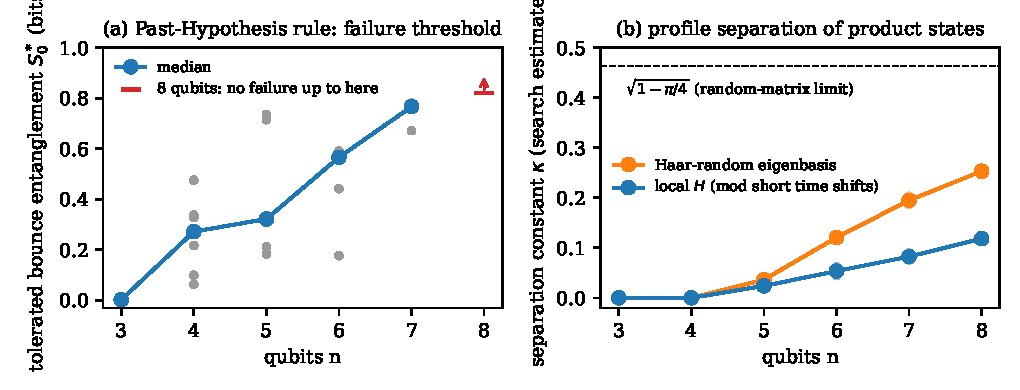
\includegraphics[width=\linewidth]{fig1.pdf}
\caption{(a) Bounce entanglement at which the product-state rule first picks a rival; grey dots are individual models. (b) Separation constant $\kappa=\inf\Hel(W(q),W(q'))/D(q,q')$ over product pairs (modulo short time translations for local $H$), estimated by search. Search estimates are \emph{upper} bounds on the true infimum. The dashed line is the Haar prediction $\sqrt{1-\pi/4}$ for orthogonal pairs.}
\label{fig:1}
\end{figure}

\paragraph{Separation constants.} Fig.~\ref{fig:1}(b) shows $\kappa=0$ at 3--4 qubits, where pairs of nearly orthogonal product states with identical profiles exist, and growth from 5 qubits on. For local $H$ the only near-degenerate directions found were short time translations. These are ``when'' ambiguities, not rival worlds, and are quotiented out.

\paragraph{Rival floor.} For an exactly unentangled bounce, Table~\ref{tab:floor} lists the lowest per-site entropy reached by any \emph{rival} reading, i.e.\ any minimum off the history. It rises steadily with $n$ for both local and Haar-random eigenbases. The rise is therefore generic, consistent with the heuristic in Sec.~\ref{sec:discussion}. The rule succeeds when the bounce's optimized entanglement lies below this floor. At 7 qubits, the optimized true-basin values at which failures set in (0.34--0.38 bits) are comparable to these floors, although the floors refer to the unperturbed bounce and the comparison is only indicative. Floors are the best rivals found, so they are upper bounds on the true floor.

\begin{table}[h]\centering\small
\begin{tabular}{ccc}
\toprule
qubits & local $H$ (two models) & Haar eigenbasis (two draws)\\
\midrule
4 & 0.056, 0.042 & 0.084, 0.035\\
5 & 0.136, 0.076 & 0.227, 0.065\\
6 & 0.284, 0.138 & 0.344, 0.359\\
7 & 0.352, 0.229 & 0.416, 0.444\\
\bottomrule
\end{tabular}
\caption{Rival floor: lowest mean single-qubit entropy (bits) among off-history minima, for an exactly unentangled bounce (40 random starts per case; 18--20 at 7 qubits).}
\label{tab:floor}
\end{table}

\paragraph{ETH-A.} For random product pairs $q'=Lq$, with $L$ a rotation on 1--4 sites, Table~\ref{tab:eth} and Fig.~\ref{fig:2} compare exact $\Hel^2$ with the ETH-A model, whose envelopes and correlations are smoothed at energy resolution 0.5. The model's error is about 3\% of $\Hel^2$ and shrinks with size. The measured gap ratio $\gamma/D^2$ has minimum 0.74 and 0.56 at 9 and 10 qubits for mid-spectrum pairs (median about 0.92). For the coldest product states of three different 10-qubit chains, near the ground-state energy, the minima are 0.45, 0.44 and 0.49. So $\gamma_0$ falls at low temperature but stays well away from zero.

\begin{table}[h]\centering\small
\begin{tabular}{ccccc}
\toprule
qubits & pairs & mean exact $\Hel^2$ & error of Haar formula & error of ETH-A model\\
\midrule
8 & 24 & 0.172 & 0.015 & 0.009\\
9 & 24 & 0.162 & 0.021 & 0.007\\
10 & 24 & 0.151 & 0.009 & 0.004\\
11 & 12 & 0.149 & 0.008 & 0.005\\
\bottomrule
\end{tabular}
\caption{Mean absolute error of the Haar formula $1-\frac\pi4F(|\braket{q}{q'}|^2)$ and of the ETH-A model against exact profile separations on generic local chains.}
\label{tab:eth}
\end{table}

\begin{figure}[h]\centering
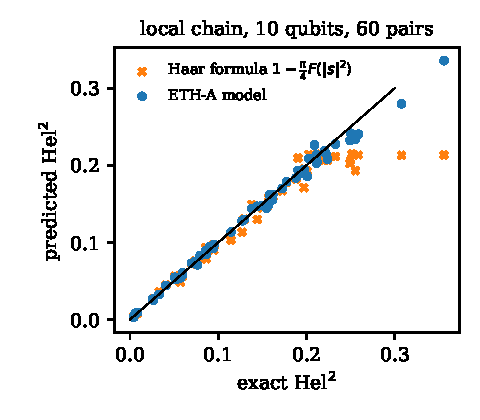
\includegraphics[width=0.48\linewidth]{fig2.pdf}
\caption{Exact versus predicted $\Hel^2$ for 60 product pairs on a 10-qubit chain (mean absolute error 0.005 for ETH-A, 0.013 for the Haar formula).}
\label{fig:2}
\end{figure}

\paragraph{Search adequacy.} Extra random starts found nothing better than the true bounce in the following checks: about 2{,}700 starts in each of two 5-qubit models; 270--290 in each of two 7-qubit models; and 165--170 for each of the two most entangled 7-qubit ground-state bounces. The weakest points are the 8-qubit perturbed bounces at $\theta=0.8$. There, 15--27 starts found no rival, but random starts rarely reached even the true basin (0--7\%), so rivals may have been missed.

\section{Local Hamiltonians: mechanism, worst cases and energy dependence}
\label{sec:toward}

\paragraph{A route through rigorous random-matrix theory.} For $H=H_{\rm loc}+\lambda W$ with $W$ a Wigner matrix, ETH and joint Gaussian fluctuations of eigenvector overlaps are theorems~\cite{CES2021,Benigni2020,CEHK2023,BenigniCipolloni2024}. Overlaps of deterministic vectors with the eigenvectors are asymptotically Gaussian, with covariance given by the imaginary part of a deterministic resolvent built from $H_{\rm loc}$. That is exactly the structure ETH-A assumes, with the correlation $c(E)$ fixed by that resolvent.
Two gaps separate this from a proof of $\mathrm{Sep}$. First, the theorems control finitely many overlaps with polynomially small failure probability, while the net argument needs all $N$ eigenvectors at once and failure probability $e^{-\Omega(n\log n)}$ per pair. Second, the published results take a deformation of bounded norm, so $H_{\rm loc}/n$ has to be treated with relatively weak noise.

\paragraph{A short-time mechanism.} The correlation $c(E)$ is built from energy-resolved matrix elements $\langle q|\delta_w(H-E)|q'\rangle$. Their Fourier transforms involve the amplitudes $\langle q|e^{-iHt}|q'\rangle$, which for product states decay on the time scale $1/\sqrt n$. At any resolution $w$ that is not exponentially small, the matrix elements are therefore governed by short-time dynamics, assuming, as ETH does, that the smooth functions do not depend on the resolution.
For states differing on a few sites, a cluster expansion suggests $\langle q|e^{-iHt}|q'\rangle\approx\langle q|q'\rangle\langle q|e^{-iHt}|q\rangle$ at those times. That gives $c(E)\approx\langle q|q'\rangle$, hence $\gamma\approx D^2$: the random-matrix value $\gamma_0=1$. This argument is heuristic.

Table~\ref{tab:deformed} tests it on random product states and partners differing on one or two sites. From 7 to 11 qubits, the mean separation matches the random-matrix prediction to within 8\%, with or without added noise; the worst of 40 pairs retains 56--84\% of it. Weak noise has no visible effect, so its role in a proof would be purely technical.
A proof along these lines would need a Berry--Esseen-type theorem for the cross-amplitudes of product states, extending Ref.~\cite{BCG2015}, together with uniform versions of the random-matrix results. Tables~\ref{tab:worst} and~\ref{tab:energy} test the prediction on worst cases and at low energy.

\begin{table}[h]\centering\small
\begin{tabular}{cccc}
\toprule
qubits & $\lambda=0$ & $\lambda=0.5$ & $\lambda=2$\\
\midrule
7 & 1.08 (0.57) & 1.07 (0.56) & 1.03 (0.64)\\
8 & 1.05 (0.70) & 1.06 (0.84) & 1.03 (0.75)\\
9 & 0.99 (0.79) & 0.99 (0.77) & 0.99 (0.82)\\
10 & 1.04 (0.67) & 1.03 (0.61) & 1.03 (0.63)\\
11 & 1.00 (0.77) & 1.00 (0.83) & 0.99 (0.82)\\
\bottomrule
\end{tabular}
\caption{Separation $\Hel^2$ of locally differing product-state pairs divided by the random-matrix prediction $1-\frac\pi4F(1-D^2)$, for $H_{\rm loc}+\lambda W$ with $W$ a GUE matrix of spectral radius 2: mean over 40 pairs (minimum in parentheses).}
\label{tab:deformed}
\end{table}

\paragraph{Worst cases.} Random pairs can miss the hardest ones, so we also searched adversarially. For each base product state, we minimized the separation ratio over all partners differing on the two middle sites, with $D^2\ge0.1$ (Table~\ref{tab:worst}).

For chaotic chains at high energy, the worst case rises steadily with size: the median is 0.46, 0.65, 0.78 and 0.91 from 6 to 12 qubits, so the gap to the random-matrix value roughly halves every two qubits. The three independent Hamiltonians at 10 qubits agree closely.
The integrable control, a random-coupling transverse-field Ising chain, is consistently lower (median 0.28, 0.47, 0.56). It does not collapse on these partners, though; a single-Hamiltonian run that suggested collapse was not representative.

Low energies are treated below.

\begin{table}[h]\centering\small
\begin{tabular}{ccc}
\toprule
qubits & chaotic, high energy & integrable, high energy\\
\midrule
6 & 0.46 (0.15--0.59) & 0.28 (0.18--0.44)\\
8 & 0.65 (0.48--0.82) & 0.47 (0.16--0.66)\\
10 & 0.78 (0.73--0.88) & 0.56 (0.35--0.68)\\
12 & 0.91 (0.87--0.93)$^\dagger$ & --\\
\bottomrule
\end{tabular}
\caption{Adversarial worst-case separation, as a fraction of the random-matrix value, for partners differing on the two middle sites. High energy: median (range) over 12 base states, 4 for each of 3 Hamiltonians. $^\dagger$One Hamiltonian, 4 base states, lighter search; at 10 qubits the lighter search raises values by at most 0.04. Search-based values are upper bounds on the true worst case.}
\label{tab:worst}
\end{table}

\paragraph{Energy dependence.} To study low energies properly, we generated many distinct product states at fixed energy fractions from random starts, using four independent chaotic Hamiltonians per size (Table~\ref{tab:energy}).
Separation weakens at low energy but improves with size at every energy tested. At 10 qubits, the median worst case is 0.60, 0.73 and 0.78 at 10\%, 25\% and 50\% of the spectrum, and the smallest values found are 0.33, 0.46 and 0.73.

Two explanations were tested on 81 further base states. Rare weak couplings that nearly isolate the modified sites do not explain the hard cases: the Spearman correlation is 0.07 ($p=0.5$).
The effective dimension $N_{\rm eff}=1/\sum_kp_k^2$ of the base state explains much of the variation (correlation 0.62, $p=5\times10^{-10}$). At 10\% of the spectrum, product states at these sizes spread over only about 4--8 energy eigenstates, against 25--430 in the middle, so low energy behaves like a much smaller system. It is not the whole story: at fixed $N_{\rm eff}$, larger systems still separate better (residual correlation with $n$ of 0.48).
At 10\% of the spectrum, $\log_2N_{\rm eff}$ grows by only about 0.3 per qubit in this range, so reaching the high-energy regime there would take much larger systems. The conjecture that chaotic local systems attain the random-matrix value is therefore well supported at high energy and plausible, but untested, at low energy. When the partner may differ on every site, the worst cases are lower. Searches from mid-spectrum and low-energy base states give 0.04--0.21 at 6 qubits, 0.24--0.30 at 8 and 0.23--0.26 at 10, with strongly entangling relating unitaries. These stay well away from zero but show no clear trend from 8 to 10 qubits, so for general partners only the weaker conjecture, a size-independent $c>0$, is supported.

\begin{table}[h]\centering\small
\begin{tabular}{cccc}
\toprule
qubits & 10\% of spectrum & 25\% & 50\%\\
\midrule
6 & 0.36 (0.13) [2.0] & 0.43 (0.21) [3.8] & 0.46 (0.15) [4.7]\\
8 & 0.57 (0.31) [2.3] & 0.61 (0.47) [4.9] & 0.65 (0.48) [6.8]\\
10 & 0.60 (0.33) [3.1] & 0.73 (0.46) [6.2] & 0.78 (0.73) [8.8]\\
\bottomrule
\end{tabular}
\caption{Worst-case separation of chaotic chains by energy: median (minimum) over 16 base states from 4 Hamiltonians (12 from 3 at 50\%), with the mean $\log_2N_{\rm eff}$ of the base states in brackets. Search-based values are upper bounds on the true worst case.}
\label{tab:energy}
\end{table}

\paragraph{Symmetries.} If $H$ commutes with a product unitary $P=\bigotimes_iP_i$ (for example a global spin flip), then $P$ is diagonal in the energy basis, so $q$ and $Pq$ have identical profiles. Such twins can be far apart ($D(q,Pq)=1$ in a 6-qubit example), so no separation constant exists. They are harmless, because $P\in\Gamma$ and $PT_0P^\dagger=T_0$: both readings describe the same division. For local Hamiltonians with symmetries, distances should therefore be taken modulo time translations and product unitaries commuting with $H$ (and, for uniform couplings, lattice symmetries, which merely relabel subsystems). The Hamiltonians in our simulations have site-dependent random couplings and no such symmetries.

\paragraph{Time reversal.} Antiunitary symmetries behave differently. If $H$ is real in a product basis, as for time-reversal-invariant Hamiltonians without magnetic fields, then every state $q$ and its complex conjugate $\bar q$ have identical profiles, and $\bar q$ is a product state whenever $q$ is. The unitary in $\Gamma$ relating them is in general entangling (operator entanglement 0.82--0.97 in our examples), so it changes the division. In that division the history reads as $\overline{\psi(-t)}$: the same history run backward. A search with partners free on all sites finds exactly these twins in real-coupled chains, with separation ratio below $10^{-9}$ at 6 and 8 qubits and each twin within $4\times10^{-5}$ of a time-shifted $\bar q$; making the couplings of a complex chain real creates them. For time-reversal-invariant Hamiltonians the residual freedom is therefore time translation together with time reversal: a single simple moment fixes the history but not its direction. Theorems~\ref{thm:exact}--\ref{thm:mps} are unaffected, since real eigenbases form a Haar-null set, and our main simulations use complex couplings. Theorem~\ref{thm:exactTR} makes this exact for generic real eigenbases. Numerically, random real bases have twins other than conjugates at 3--4 qubits and none from 5 qubits on: the minimum of $\Hel^2/D^2$, with distance taken modulo conjugation, is 0.002--0.003 at 5 qubits and 0.013--0.047 at 7, matching complex bases. In real-coupled chaotic chains, an all-sites search excluding time shifts and time reversal finds worst ratios of 0.06--0.13 at 6--8 qubits, nonzero but lower than for complex chains.

\paragraph{The exact problem is algebraic but large.} For nondegenerate $H$, two states share an energy profile if and only if they share the moments $\langle H^j\rangle$ for $j=1,\dots,N-1$. For product states each moment is affine in every site's Bloch vector. Twins of a given local $H$ are therefore the off-diagonal real solutions of $N-1$ multilinear equations in $4n$ unknowns, and the set of couplings admitting twins is semi-algebraic. This makes exact discrimination at fixed $n$ a finite problem, but not a tractable one. A square subsystem has a multihomogeneous B\'ezout number of about $10^{15}$ at 5 qubits and $10^{20}$ at 6, far beyond certified homotopy continuation. Nor does the argument of Ref.~\cite{CPR2019}, that one good example implies almost all, transfer directly. It applies to properties defined by rank conditions, while absence of twins is global. Dimension counting in the style of Kech and Wolf needs a family rich enough to move every pair of states independently: Haar bases have $N^2$ parameters, local Hamiltonians $O(n)$. This is the technical core of why locality makes the problem hard.

\section{Discussion}
\label{sec:discussion}

\paragraph{Relation to the Entanglement Past Hypothesis.} Al-Khalili and Chen~\cite{AlKhaliliChen2024} formulate an Entanglement Past Hypothesis: the early universe had low entanglement entropy relative to a factorization. They treat the dependence on a factorization as a difficulty and consider factorization-independent versions. One of these requires low entanglement on \emph{every} factorization in a class $R$, such as partitions of space. They also note an apparent circularity: specifying $R$ by spatial structure conflicts with deriving space from entanglement.

Our rule runs in the opposite direction. We take $R$ to be the divisions in which $H$ is equally local, which is determined by $(H,\psi)$ alone, and quantify existentially: the selected division is the one in $R$ in which some moment of the history is simple. By Theorem~\ref{thm:exact}, for generic eigenbases and $n\ge5$, a bounce with full energy support is unentangled in only one member of $R$. So the universal version fails for this class, while the existential version selects the division.
This removes the circularity for locality-preserving divisions, at the cost of assuming that $H$ is local in some division. The locality constraint is also what gives the rule content. Rovelli~\cite{Rovelli2014} observed that without any constraint, a low-entropy past is trivial: for a generic state there is always some split in which entropy starts low and grows.

\paragraph{Direction of time.} For time-reversal-invariant Hamiltonians the rule fixes the history and its division into subsystems, but not the direction of time: the simple moment looks the same from either side. This fits the picture of Barbour, Koslowski and Mercati, in which solutions of a time-symmetric gravitational model divide at a unique ``Janus point'', with arrows of time pointing away from it in both directions~\cite{BKM2014}, and the two-arrow cosmology of Carroll and Chen~\cite{CarrollChen2004}. On this reading the simple moment determines what the parts are, while the direction of time is set on each side by entropy growing away from it. We have not found this connection made elsewhere, but have not searched exhaustively.

\paragraph{Objections.} (i) \emph{Simplicity smuggles in structure.} The rule is an invariant property of $(H,\psi,T)$ (Lemma~\ref{lem:invariance}), close to the Entanglement Past Hypothesis. It is, however, a stronger and more specific postulate than low thermodynamic entropy. A critic can fairly say that we have not derived subsystem structure from the Past Hypothesis, but introduced a simplicity postulate and shown that it identifies a factorization. We accept that description. The content of the result is that this postulate, unlike simplicity without the locality constraint, is unambiguous. (ii) \emph{Stoica showed the Past Hypothesis cannot give uniqueness.} He considered it as a way to reduce the candidate structures and concluded that, because its constraints are unitarily invariant, infinitely many choices remain~\cite[Sec.~VII.B]{Stoica2022}. We agree: the rule leaves infinitely many divisions, but they are exactly the history's time translates. Stoica notes that if only time translation remained, a unique four-dimensional spacetime could be recovered in place of a unique three-dimensional space, turning non-uniqueness into a feature (Remark~10). He then raises objections to that hope for Hamiltonians whose time orbits are dense (Remark~11). In Sec.~VII.E he observes that restricting the physical states to a single orbit $\{e^{-iHt}\psi_0\}$ gives a unique spacetime, given an emergent notion of three-dimensional space, but calls this restriction ad hoc and asks for a derivation from physical principles. Our result can be read as such a derivation: the Past Hypothesis, together with locality, selects that orbit. Because the selected divisions are the time translates themselves, parametrized by $t$, they come with the ordering that Remark~11 finds missing for dense orbits. In later work Stoica argues that HSF cannot account for observed change at all~\cite{Stoica2026}; we do not settle that question, and the rule does not select a ``now''. (iii) \emph{Random eigenbases are unphysical.} Proposition~\ref{prop:coarse} shows that some eigenvector-level hypothesis is unavoidable for local $H$. ETH-A is a random-amplitude version of the standard eigenstate thermalization hypothesis, and it matches our data at 8--11 qubits. (iv) \emph{The simulations are small.} They test the predicted thresholds and the model where testing is possible. For random eigenbases the claims about large systems rest on the theorems; for local Hamiltonians they remain conjectural.

\paragraph{Scope.} We work inside finite-dimensional HSF with a non-degenerate spectrum and do not defend the framework. The rule does not select a ``now''. Degenerate spectra, continuous spectra and field theory are not treated.

\paragraph{Open problems.} (1) Prove $\mathrm{Sep}$, modulo time translations, symmetries and, for time-reversal-invariant $H$, time reversal, for chaotic local Hamiltonians under assumptions weaker than ETH-A, for instance design-like properties of eigenvectors within energy shells. Even the exact version (no twins for almost every choice of local couplings) is open. (2) Explain why the tolerance measured in \emph{per-site} entanglement grows with $n$ (Table~\ref{tab:rule}), which the global bounds do not capture. A heuristic in the Haar model points to the mechanism. For a fixed $\varphi$, invariance under unitaries fixing $\psi_0$ makes the reading $V_\varphi^\dagger\psi_0=z\psi_0+\sqrt{1-|z|^2}\,\xi$, with $\xi$ Haar-random in $\psi_0^\perp$. Away from the bounce ($|z|$ small), its $n$ single-site Bloch vectors are then approximately independent with variance $O(1/N)$. The probability that all of them have squared length at least $\rho$ would decay like $e^{-cnN\rho}$, while a net of the fibre has only $e^{O(N\log(1/\rho))}$ points. That suggests no rival can exceed per-site purity excess $\rho\gtrsim\log n/n$, so the rival floor approaches the maximally mixed value. Making this rigorous requires controlling correlations between single-site marginals, which become strong near product states. (3) Settle the status of the constants $\gamma_0(\beta)$ at low temperature.

\section*{Acknowledgements and disclosure of AI use}
[To be completed by the authors.] This work was carried out in an extended interactive session with the AI system Claude (Anthropic). The AI proposed the main constructions, proved the stated results, wrote and ran all numerical code, and produced a first draft of this manuscript. [State here which proofs and computations were independently verified, by whom, and how.] Responsibility for all content rests with the human authors.

\section*{Code and data availability}\sloppy
All scripts and raw results are provided with this manuscript: \texttt{past\_hypothesis\_scan.py}, \texttt{mps\_rule\_scan.py}, \texttt{separation\_constant.py}, \texttt{eth\_check.py}, \texttt{random\_matrix\_prediction.py}, \texttt{mereology\_toy\_model.py} and \texttt{past\_hypothesis\_raw\_results.tar.gz}.

\appendix
\section{Proofs}
\label{app:proofs}

\begin{lemma}\label{lem:helD}
For any states, $\Hel(W(\phi),W(\phi'))\le D(\phi,\phi')$.
\end{lemma}
\begin{proof}
$\sum_k|\braket{k}{\phi}||\braket{k}{\phi'}|\ge|\braket{\phi}{\phi'}|$, so $\Hel^2\le1-|\braket{\phi}{\phi'}|\le1-|\braket{\phi}{\phi'}|^2$.
\end{proof}

\begin{lemma}[Exact expectation]\label{lem:expect}
Let $m,m'$ be unit vectors with $|\braket{m}{m'}|=s$, and let $\{\ket{u_k}\}$ be the columns of a Haar-random $U\in U(N)$. Then, at every $N$,
\[
\E\sum_{k=1}^N|\braket{u_k}{m}||\braket{u_k}{m'}|=\frac\pi4F(s^2),\qquad F={}_2F_1(-\tfrac12,-\tfrac12;1;\cdot),
\]
and consequently $1-\E\sum_k|\braket{u_k}{m}||\braket{u_k}{m'}|\ge(1-\pi/4)(1-s^2)$.
\end{lemma}
\begin{proof}
Write $m'=e^{i\alpha}(s\,m+c\,m_\perp)$ with $c=\sqrt{1-s^2}$ and $m_\perp\perp m$. Each column $u_k$ is uniform on the sphere, so $(\braket{u_k}{m},\braket{u_k}{m_\perp})$ has the law of $(\bar g_1,\bar g_2)/\|g\|$ for a standard complex Gaussian vector $g\in\mathbb C^N$ with $\E|g_i|^2=1$. The direction $g/\|g\|$ is independent of $\|g\|$, and $\E\|g\|^2=N$. The integrand is homogeneous of degree 2, so $\E[|x_1||sx_1+cx_2|]=N^{-1}\E|g_1||sg_1+cg_2|$. It remains to show $\E|X||Y|=\frac\pi4F(s^2)$ for $X=g_1$, $Y=sg_1+cg_2$. Conditionally on $X$, $Y$ is complex Gaussian with mean $sX$ and variance $c^2$, so $|Y|$ is Rice-distributed with $\E[|Y|\,|\,X]=c\frac{\sqrt\pi}{2}\,{}_1F_1(-\tfrac12;1;-s^2|X|^2/c^2)$. With $u=|X|^2\sim\mathrm{Exp}(1)$ and the Laplace transform $\int_0^\infty u^{b-1}e^{-u}{}_1F_1(a;1;-ku)\,du=\Gamma(b)\,{}_2F_1(a,b;1;-k)$, $\E|X||Y|=c\frac\pi4\,{}_2F_1(-\tfrac12,\tfrac32;1;-s^2/c^2)$. Pfaff's transformation ${}_2F_1(a,b;c;z)=(1-z)^{-a}{}_2F_1(a,c-b;c;\frac{z}{z-1})$ with $z=-s^2/c^2$ gives $(1-z)^{1/2}=1/c$ and $z/(z-1)=s^2$, hence $\E|X||Y|=\frac\pi4F(s^2)$; the case $s=1$ follows by continuity. Summing over $k$ gives the first claim. For the second, $F$ has positive Taylor coefficients, so it is convex, and Gauss's theorem gives $F(1)=4/\pi$. The function $G(x)=\frac\pi4(1-F(x))+(1-\frac\pi4)x$ is therefore concave with $G(0)=G(1)=0$, hence $G\ge0$ on $[0,1]$.
\end{proof}

\begin{lemma}[Lipschitz bounds and concentration]\label{lem:conc}
Let $g_{m,m'}(U)=\sum_k|\braket{u_k}{m}||\braket{u_k}{m'}|$. Then $|g(U)-g(U')|\le2\|U-U'\|_{\rm HS}$, hence $\Pr[g\ge\E g+t]\le e^{-Nt^2/48}$. Moreover $|g_{m,m'}-g_{\tilde m,\tilde m'}|\le\sqrt2\,\big(D(m,\tilde m)+D(m',\tilde m')\big)$ for every $U$.
\end{lemma}
\begin{proof}
By the triangle and Cauchy--Schwarz inequalities, $|g(U)-g(U')|\le\|(U-U')^\dagger m\|+\|(U-U')^\dagger m'\|\le2\|U-U'\|_{\rm op}\le2\|U-U'\|_{\rm HS}$. For Haar-distributed $U\in U(N)$ with the Hilbert--Schmidt metric, every $L$-Lipschitz function satisfies $\Pr[f\ge\E f+t]\le e^{-Nt^2/(12L^2)}$~\cite[Cor.~17]{MeckesMeckes2013}; see also~\cite[Ch.~5]{Meckes2019}. For the last claim, $|g_{m,m'}-g_{\tilde m,m'}|\le\min_\varphi\|m-e^{i\varphi}\tilde m\|=\sqrt{2-2|\braket{m}{\tilde m}|}\le\sqrt2\,D(m,\tilde m)$.
\end{proof}

\begin{lemma}[Nets]\label{lem:nets}
For $0<\delta\le1$, $\Prod$ has a $\delta$-net in $D$ of size at most $(2n/\delta)^{3n}$, and $\MPS_\chi$ has one of size at most $(5n/\delta)^{4n\chi^2}$.
\end{lemma}
\begin{proof}
For product states, $D(\otimes_i q_i,\otimes_i\tilde q_i)\le\sum_iD(q_i,\tilde q_i)$ by subadditivity of the trace distance under tensor products, and $D=|r-\tilde r|/2$ for Bloch vectors. A $(2\delta/n)$-net of the unit sphere in $\mathbb R^3$ has at most $(1+n/\delta)^3\le(2n/\delta)^3$ points; take products. For MPS in left-canonical form, $\psi$ is a product of isometries $V_i$, each with real dimension at most $4\chi^2$. Take as net a maximal $\epsilon'$-separated subset of the isometries themselves, which is an $\epsilon'$-net in operator norm consisting of isometries. Balls of radius $\epsilon'/2$ about its points are disjoint and lie in the operator-norm ball of radius $1+\epsilon'/2$, so it has at most $(1+2/\epsilon')^{4\chi^2}\le(5/\epsilon')^{4\chi^2}$ points. Because the net points are isometries, every net state $\tilde\psi$ is a normalized MPS in left-canonical form, and every factor in both chains has operator norm 1. Telescoping then gives $\|\psi-\tilde\psi\|\le\sum_i\|V_i-\tilde V_i\|_{\rm op}$, and $D\le\|\psi-\tilde\psi\|$ for unit vectors. Take $\epsilon'=\delta/n$.
\end{proof}

\begin{proof}[Proof of Theorems~\ref{thm:haar} and~\ref{thm:mps}]
Set $\epsilon=0.1r_0^2$, $t=\epsilon/2$ and $\delta=\epsilon/(8\sqrt2)$, and let $\mathcal N$ be the net of Lemma~\ref{lem:nets}. By Lemma~\ref{lem:conc} and a union bound, with probability at least $1-|\mathcal N|^2e^{-Nt^2/48}$ every net pair satisfies $g\le\E g+t$. Every pair lies within $\delta$ of a net pair in each argument, and $g$ and $\E g$ each move by at most $2\sqrt2\,\delta$. So on this event $g\le\E g+t+4\sqrt2\,\delta=\E g+\epsilon$ for all pairs. By Lemma~\ref{lem:expect}, every pair with $D\ge r_0$ then has $\Hel^2=1-g\ge(1-\pi/4)r_0^2-0.1r_0^2\ge0.114\,r_0^2$. Inserting $|\mathcal N|^2\le(16\sqrt2\,n/\epsilon)^{6n}$ for products, or $(40\sqrt2\,n/\epsilon)^{8n\chi^2}$ for MPS, and $Nt^2/48=2^nr_0^4/19200$, gives the stated probabilities. Finally, $\eta\le0.16r_0$ implies $2\eta<\sqrt{0.114}\,r_0$, so Lemma~\ref{lem:robust} applies.
\end{proof}



\begin{proof}[Proof of Theorem~\ref{thm:exactTR}]
For a real unit vector $o$ and $m=a+ib$ with $a,b$ real, $|\langle o|m\rangle|^2=o^{\mathsf T}(aa^{\mathsf T}+bb^{\mathsf T})o=o^{\mathsf T}\,\mathrm{Re}(mm^\dagger)\,o$. So $m$ and $m'$ share a profile in the real basis $O=(o_1,\dots,o_N)$ if and only if $\Phi(O):=\mathrm{diag}(O^{\mathsf T}AO)=0$, where $A=\mathrm{Re}(mm^\dagger)-\mathrm{Re}(m'm'^\dagger)$ is real symmetric and traceless.

\emph{$A=0$ exactly for the stated twins.} $A=0$ means $aa^{\mathsf T}+bb^{\mathsf T}=a'a'^{\mathsf T}+b'b'^{\mathsf T}$, so $(a',b')=(a,b)R$ for some $R\in O(2)$. Rotations give $m'=e^{i\alpha}m$ and reflections give $m'=e^{i\alpha}\bar m$; if $a,b$ are dependent, $m$ is real up to phase and the two cases coincide.

\emph{For $A\ne0$ the fibre $\Phi^{-1}(0)$ has codimension at least $N-1$ in $O(N)$.} With $B=O^{\mathsf T}AO$ and $X$ skew-symmetric, $d\Phi_O(OX)=\mathrm{diag}([B,X])$, and each pair $j<k$ contributes $2B_{jk}X_{jk}(e_k-e_j)$. Hence $\mathrm{rank}\,d\Phi_O=N-c(B)$, where $c(B)$ is the number of connected components of the graph with edges $\{j,k\}$ for $B_{jk}\ne0$. Where the graph is connected, $\Phi$ is a submersion onto the hyperplane $\sum_kx_k=0$ and the fibre has codimension $N-1$. Where it is disconnected, the columns indexed by a component $I$ (complement $J$) span an $A$-invariant subspace $W\oplus K$, with $W$ in the range of $A$ ($\dim W=w$, $\operatorname{rank}A=r\ge1$) and $K$ in its kernel. The conditions $B_{IJ}=0$ then have codimension $w|J|+(r-w)|I|-w(r-w)$, and the diagonal conditions not already implied add at least $N-2$, or $|J|-1$ when $w=0$ (and $|I|-1$ when $w=r$). In every case the total is at least $N-1$. This parameter count assumes the remaining diagonal conditions are independent within the stratum; we have checked this step less carefully than the others, and it is the first a referee should examine.

\emph{Conclusion.} The incidence set $\{(O,m,m'):A\ne0,\ \Phi(O)=0\}$ is semi-algebraic, of dimension at most $\dim O(N)-(N-1)+2d<\dim O(N)$. Its projection to $O(N)$ therefore has lower dimension and is Haar-null, and outside it profile equality in $\mathcal S$ forces $A=0$. For the statement about divisions, argue as in Theorem~\ref{thm:exact}. If $V^\dagger\psi(t)=e^{i\alpha}\bar\psi_0$, then, because $H$ is real, $V^\dagger\psi(t+s)=e^{i\alpha}e^{-iHs}\bar\psi_0=e^{i\alpha}\,\overline{\psi(t_0-s)}$.
\end{proof}

\section{Verification record}
\label{app:verify}
Every claim that can be checked by computation was re-checked independently of the original derivations, using numerical tests, adversarial searches for counterexamples, exact or 30-digit arithmetic, and recomputation from raw data. Scripts and logs are in the code bundle.

\begin{center}\small
\begin{tabular}{p{4.4cm}p{6.6cm}p{3.2cm}}
\toprule
Claim & Check & Result\\
\midrule
Lemma~\ref{lem:fibre}, locality in $T_V$ & both inclusions on random instances & pass\\
Lemma~\ref{lem:helD} ($\Hel\le D$) & 12{,}000 random pairs and adversarial maximization of $\Hel-D$, $N=2$--$32$ & max $-2\times10^{-8}$\\
Lemma~\ref{lem:expect}, identity & Haar sampling at $N=2,3,4,8$ (12 cases); end-to-end quadrature & within sampling error; 12 digits\\
Lemma~\ref{lem:expect}, derivation steps & Rice mean, Laplace transform and Pfaff step in 30-digit arithmetic & agree to $10^{-15}$\\
$G\ge0$, convexity, $F(1)=4/\pi$, chord bound & $2\times10^5$-point grid; Taylor coefficients; closed form & pass\\
Lemma~\ref{lem:conc}, Lipschitz constants & random perturbations of $U$ and of states & max ratios 0.64 ($\le2$), 0.71 ($\le\sqrt2$)\\
Lemma~\ref{lem:conc}, concentration & statement checked against Ref.~\cite{MeckesMeckes2013}, Cor.~17 & matches\\
Lemma~\ref{lem:nets} ingredients & subadditivity, Bloch relation, $D\le\|\cdot\|$, MPS telescoping (300 chains) & pass\\
Theorems~\ref{thm:haar},~\ref{thm:mps}, constants & exact arithmetic of every constant; non-triviality threshold & pass\\
Theorem~\ref{thm:exact}, input & Kech--Wolf statement checked against the source abstract & matches\\
Dimension $8n-10$ for $\chi=2$ MPS & Jacobian rank of the MPS map, $n=3$--$8$ & exact match\\
Lemma~\ref{lem:robust}, history claim & distance independent of shift $s$ & spread $4\times10^{-16}$\\
Proposition~\ref{prop:eth}, inequalities & 20{,}000 random envelope and correlation profiles & pass\\
``Chaotic'' test Hamiltonians & mean level-spacing ratio (GUE 0.600) & 0.587, 0.599\\
Tables~\ref{tab:rule},~\ref{tab:mps},~\ref{tab:eth},~\ref{tab:floor}; Remark~\ref{rem:time} & recomputed from raw data or deterministic reruns & match after corrections\\
\bottomrule
\end{tabular}
\end{center}

\paragraph{External AI review.} The mathematics (Sections 2--5 and Appendix~\ref{app:proofs}) was reviewed by an AI model from a different developer, in two rounds. In the second round it verified Lemmas~\ref{lem:expect}, \ref{lem:conc} and~\ref{lem:robust}, the constants and proof of Theorem~\ref{thm:haar}, Theorem~\ref{thm:exact}, and the expectation bound of Proposition~\ref{prop:eth}. It reversed two objections from its first round (to the concentration step and to the sign of the $\pi/4$ bound) after they were tested numerically. It identified four problems, all now addressed: the MPS net was not stated to consist of isometries; Proposition~\ref{prop:coarse} omitted hypotheses of the Berry--Esseen theorem; the state space in Theorem~\ref{thm:exact} needed specifying; and a claim about infinite temperature needed an extra assumption. A third round confirmed the repairs, and on its suggestion the unproven uniform step of Proposition~\ref{prop:eth} was moved out of the proposition into Remark~\ref{rem:ethuniform}. It also asked for a sharper separation between the random-eigenbasis theorems and the local-Hamiltonian results, now stated at the start of Section~\ref{sec:local}. An AI review is not an expert review: models can share blind spots, so this is a screen, not a verification.

\paragraph{Errors found and corrected in this pass.} The ground-state entanglement range (0.03 corrected to 0.08 bits); two table ranges (0.02 to 0.01 at 3 qubits, 0.19 to 0.18 at 5 qubits); the non-triviality threshold ($n\approx24$ corrected to $n=25$); the optimistic-constants estimate (15 corrected to 19); an ``exactly when'' statement in Sec.~\ref{sec:reduction} that needed ``for every bounce''; a claim that the rule fails below the dimension thresholds, which holds only for perturbed bounces; and the concentration step of Proposition~\ref{prop:eth}, now labelled a sketch. Two initial test failures were errors in the test code (a tolerance below floating-point precision and unnormalized test states), not in the paper.

\paragraph{Reference audit.} Every cited work was checked to exist and to say what it is cited for. This found one wrong author name (Dulani, not Dulaney), one placeholder title, and missing publication details, all corrected. It also found related work that had not been cited~\cite{ZLL2004,Zanardi2024,Adil2024}, now added. The passages of Stoica's paper discussed in Sec.~\ref{sec:discussion} (Secs.~VII.B and VII.E, Remarks~10 and~11) were checked against version~9 of the arXiv preprint. That check corrected an overstated paraphrase and showed that Stoica first proposed the Past Hypothesis as a selection principle, which is now credited.

\paragraph{Not verifiable by computation here.} The proofs of the cited theorems (Kech--Wolf; Meckes--Meckes; the Berry--Esseen theorem of Brand\~ao, Cramer and Gu\c{t}\u{a}; the area laws of Hastings and of Arad \emph{et al.}); the remaining bibliographic details marked in the source; novelty; and the search-based quantities (separation constants and search-adequacy counts), which depend on time-budgeted random searches and are reported from logs. These, and the proofs as a whole, still require independent expert review.

\paragraph{Counterexample search.} A later search with partners free on all sites found exact twins in time-reversal-invariant chains. They are time-reversed readings of the same history, discussed in Sec.~\ref{sec:toward}. It found no twins in complex-coupled chaotic chains, where the worst cases stay at 0.23--0.30 of the random-matrix value at 8--10 qubits. Theorem~\ref{thm:exactTR} and its proof were added after the external reviews and have not been reviewed; the threshold it predicts was checked numerically.

\section{Numerical methods}
\label{app:numerics}

The Hamiltonian is $H=\sum_i\sum_a h_{i,a}\sigma^a_i+0.7\sum_i\sum_{a,b}J_{i,ab}\sigma^a_i\sigma^b_{i+1}$, with independent standard normal couplings and a seed per model. Seeds are small consecutive integers recorded in the code, so every table can be regenerated and extended to other seeds. Eigenvectors come from exact diagonalization. For the product rule, the smooth objective is the mean single-qubit linear entropy of $V^\dagger\psi_0$, and results are reported in von Neumann entropy. For the MPS rule, the objective is $\sum_{\rm cuts}(1-\sum_{j\le\chi}s_j^2)$, whose gradient is $-2\,\mathrm{Re}$ of the overlap with the truncated state at each cut. Both objectives are optimized over $\varphi\in[0,2\pi)^N$ with BFGS from the identity (the true basin) and from 6--2{,}700 random starts, depending on size. A threshold is the midpoint between the last bounce entanglement at which every tested point picked the history and the first at which one did not. Separation constants minimize $\Hel/D$ (or $\Hel/D_T$, with $D_T$ minimized over $|t|\le0.6$) over pairs of product states by L-BFGS from random starts. The ETH-A model uses envelopes and correlations smoothed with a Gaussian kernel of width 0.5 in energy.

\begin{thebibliography}{99}
\bibitem{BKM2014} J.~Barbour, T.~Koslowski and F.~Mercati, Identification of a gravitational arrow of time, Phys.\ Rev.\ Lett.\ \textbf{113}, 181101 (2014), arXiv:1409.0917.
\bibitem{CarrollChen2004} S.~M. Carroll and J.~Chen, Spontaneous inflation and the origin of the arrow of time, arXiv:hep-th/0410270 (2004).
\bibitem{AlKhaliliChen2024} J.~Al-Khalili and E.~K. Chen, The decoherent arrow of time and the entanglement past hypothesis, arXiv:2405.03418 (2024). % verify journal version
\bibitem{Rovelli2014} C.~Rovelli, Why do we remember the past and not the future? The `time oriented coarse graining' hypothesis, arXiv:1407.3384 (2014).
\bibitem{CarrollSingh2021} S.~M. Carroll and A.~Singh, Quantum mereology: factorizing Hilbert space into subsystems with quasiclassical dynamics, Phys.\ Rev.\ A \textbf{103}, 022213 (2021), arXiv:2005.12938.
\bibitem{Stoica2022} O.~C. Stoica, 3D-space and the preferred basis cannot uniquely emerge from the quantum structure, arXiv:2102.08620 (v9, 2024); to appear in Adv.\ Theor.\ Math.\ Phys.
\bibitem{Stoica2024} O.~C. Stoica, Does the Hamiltonian determine the tensor product structure and the 3d space?, arXiv:2401.01793 (2024).
\bibitem{Stoica2026} O.~C. Stoica, No change in Hilbert space fundamentalism, arXiv:2602.20331 (2026).
\bibitem{Stoica2026comment} O.~C. Stoica, Comment on ``On the emergence of preferred structures in quantum theory'' by Soulas, Franzmann, and Di Biagio, arXiv:2603.07674 (2026).
\bibitem{Soulas2025} A.~Soulas, G.~Franzmann and A.~Di Biagio, On the emergence of preferred structures in quantum theory, arXiv:2512.07468 (2025).
\bibitem{ZLL2004} P.~Zanardi, D.~A. Lidar and S.~Lloyd, Quantum tensor product structures are observable induced, Phys.\ Rev.\ Lett.\ \textbf{92}, 060402 (2004).
\bibitem{Zanardi2024} P.~Zanardi, E.~Dallas, F.~Andreadakis and S.~Lloyd, Operational quantum mereology and minimal scrambling, Quantum \textbf{8}, 1406 (2024), arXiv:2212.14340.
\bibitem{Adil2024} A.~Adil, M.~S. Rudolph, A.~Arrasmith, Z.~Holmes, A.~Albrecht and A.~Sornborger, A search for classical subsystems in quantum worlds, arXiv:2403.10895 (2024).
\bibitem{CPR2019} J.~S. Cotler, G.~R. Penington and D.~H. Ranard, Locality from the spectrum, arXiv:1702.06142; Commun.\ Math.\ Phys.\ \textbf{368}, 1267 (2019).
\bibitem{CDD2026} S.~M. Carroll, N.~Diachenko and S.~Dulani, Toward a phenomenologically acceptable quantum cyclic universe, arXiv:2605.30405 (2026).
\bibitem{HMW2013} T.~Heinosaari, L.~Mazzarella and M.~M. Wolf, Quantum tomography under prior information, Commun.\ Math.\ Phys.\ \textbf{318}, 355 (2013), arXiv:1109.5478.
\bibitem{KechWolf2017} M.~Kech and M.~M. Wolf, Constrained quantum tomography of semi-algebraic sets with applications to low-rank matrix recovery, Inf.\ Inference \textbf{6}, 171 (2017), arXiv:1507.00903.
\bibitem{BCE2006} R.~Balan, P.~Casazza and D.~Edidin, On signal reconstruction without phase, Appl.\ Comput.\ Harmon.\ Anal.\ \textbf{20}, 345 (2006).
\bibitem{ABDE2025} T.~Amir, T.~Bendory, N.~Dym and D.~Edidin, The stability of generalized phase retrieval problem over compact groups, Appl.\ Comput.\ Harmon.\ Anal.\ \textbf{82}, 101838 (2026), arXiv:2505.04190.
\bibitem{Hastings2007} M.~B. Hastings, An area law for one-dimensional quantum systems, J.\ Stat.\ Mech.\ P08024 (2007).
\bibitem{AKLV2013} I.~Arad, A.~Kitaev, Z.~Landau and U.~Vazirani, An area law and sub-exponential algorithm for 1D systems, in Proc.\ ITCS (2013), arXiv:1301.1162.
\bibitem{CES2021} G.~Cipolloni, L.~Erd\H{o}s and D.~Schr\"oder, Eigenstate thermalization hypothesis for Wigner matrices, Commun.\ Math.\ Phys.\ \textbf{388}, 1005 (2021).
\bibitem{Benigni2020} L.~Benigni, Eigenvectors distribution and quantum unique ergodicity for deformed Wigner matrices, Ann.\ Inst.\ H.\ Poincar\'e Probab.\ Statist.\ \textbf{56}, 2822 (2020).
\bibitem{CEHK2023} G.~Cipolloni, L.~Erd\H{o}s, J.~Henheik and O.~Kolupaiev, Gaussian fluctuations in the equipartition principle for Wigner matrices, Forum Math.\ Sigma \textbf{11}, e74 (2023).
\bibitem{BenigniCipolloni2024} L.~Benigni and G.~Cipolloni, Fluctuations of eigenvector overlaps and the Berry conjecture for Wigner matrices, Electron.\ J.\ Probab.\ \textbf{29} (2024).
\bibitem{BerryEsseen2026} A Berry--Esseen bound for quantum lattice systems, arXiv:2605.03829 (2026). % verify authors
\bibitem{BCG2015} F.~G.~S.~L. Brand\~ao, M.~Cramer and M.~Gu\c{t}\u{a}, A Berry--Esseen theorem for quantum lattice systems and the equivalence of statistical mechanical ensembles, QIP 2015.
\bibitem{BrandaoCramer2015} F.~G.~S.~L. Brand\~ao and M.~Cramer, Equivalence of statistical mechanical ensembles for non-critical quantum systems, arXiv:1502.03263 (2015).
\bibitem{Deutsch1991} J.~M. Deutsch, Quantum statistical mechanics in a closed system, Phys.\ Rev.\ A \textbf{43}, 2046 (1991).
\bibitem{Srednicki1994} M.~Srednicki, Chaos and quantum thermalization, Phys.\ Rev.\ E \textbf{50}, 888 (1994).
\bibitem{MeckesMeckes2013} E.~S. Meckes and M.~W. Meckes, Spectral measures of powers of random matrices, arXiv:1210.2681; Electron.\ Commun.\ Probab.\ \textbf{18}, no.~78 (2013). % verify journal details
\bibitem{LoizeauSels2024} N.~Loizeau and D.~Sels, Quantum mereology and subsystems from the spectrum, Found.\ Phys.\ (2024), doi:10.1007/s10701-024-00813-2, arXiv:2409.01391.
\bibitem{Cao2026} C.~Cao, O.~Friedrich, M.~Girard, N.~Loizeau and A.~Singh, Wave packets from the spectrum, arXiv:2606.10004 (2026).
\bibitem{Kushwaha2026} V.~Kushwaha, N.~Loizeau, A.~Grinbaum and O.~Friedrich, Causality from the spectrum: emergence of causal order from process-matrix mereology, arXiv:2607.15345 (2026).
\bibitem{Meckes2019} E.~S. Meckes, \emph{The Random Matrix Theory of the Classical Compact Groups} (Cambridge University Press, 2019), Ch.~5.
\end{thebibliography}
\end{document}
